\documentclass[twoside]{article}
\usepackage{graphicx}
\usepackage{polski}
\usepackage{fancyhdr}
\usepackage{lastpage}
\usepackage{epigraph}
\usepackage{listings}
\usepackage{soul}
\usepackage{color}
\usepackage{multirow}
\usepackage{subcaption}
\usepackage{fancyvrb}
\usepackage{hyperref}
\usepackage{minted}
\usepackage{chngpage}
\usepackage{amsmath}
\usepackage{amssymb}


\title{AiSD Ex. 5., zadania}
\author{\hl{Mateusz Kamieniecki}}
\date{\today}

\lstset{
    numbers=left
}

\makeatletter

\begin{document}

\pagestyle{fancy}
\fancyhead{}
\fancyhead[L]{\@title}
\fancyhead[R]{\@author}
\fancyhead[C]{\@date}

\cfoot{\thepage\ / \pageref{LastPage}}


\newpage
\section{Zadania}


\subsubsection{Pytania, żeby się nie nudzić w trakcie zajęć}
\label{section:questions_v2}

\textbf{1.} Czy na drzewie binarnym, które nie jest regularne, można zbudować kod prefiksowy? 
Czy taki kod może być optymalny?
Proszę uzasadnić odpowiedź.

\hl{Miejsce na odpowiedzi (na temat, ale krótko):}
Można, ale nie będzie optymalny. Jak przypisujemy 0 na lewo a 1 na prawo to
dalej będzie zbudowany kod prefiksowy, ale nie będzie optymalny bo np, gdy mamy
węzeł v i syn v, to możemy usunąć v i przypiąć w do rodzica v. Wtedy kodowane
słowo jest o 1 krótsze na ścieżce i poprawiliśmy kodowanie.
\newline

\textbf{2.} Proszę wyliczyć koszt drzewa powstałego (analogicznie do przykładu z~zajęć) dla ciągu znaków 
(przecinki i spacje również należy uwzględnić; wielkość liter proszę pominąć):
\textit{Więc jeszcze seta, znakomicie 
Padniemy, ale zgódźcie się 
Że z tylu różnych dróg przez życie
Każdy ma prawo wybrać źle}.

\hl{Miejsce na odpowiedź (obliczenia + opcjonalnie rysunek / zdjęcie wynikowego drzewa):}
Najpierw trzeba wyliczyć cęstotliwość występowania znaków w tekście:

\begin{center}
\begin{tabular}{|c|c|c|c|c|c|}
\hline
symbol & \textvisiblespace & e & a & i & z \\ \hline
liczba & 19 & 11 & 8 & 7 & 7 \\ \hline
\end{tabular}

\vspace{2mm}

\begin{tabular}{|c|c|c|c|c|c|c|c|c|c|c|c|c|c|c|c|}
\hline
symbol & c & y & r & d & ż & w & s & n & m & p & l & ó & ę & t & , \\ \hline
liczba & 6 & 6 & 5 & 4 & 4 & 3 & 3 & 3 & 3 & 3 & 3 & 3 & 2 & 2 & 2 \\ \hline
\end{tabular}

\vspace{2mm}

\begin{tabular}{|c|c|c|c|c|c|c|c|c|c|c|}
\hline
symbol & k & o & g & ź & j & u & h & b & ć & . \\ \hline
liczba & 2 & 2 & 2 & 2 & 1 & 1 & 1 & 1 & 1 & 1 \\ \hline
\end{tabular}

\end{center}

\begin{figure}[h]
    \centering
    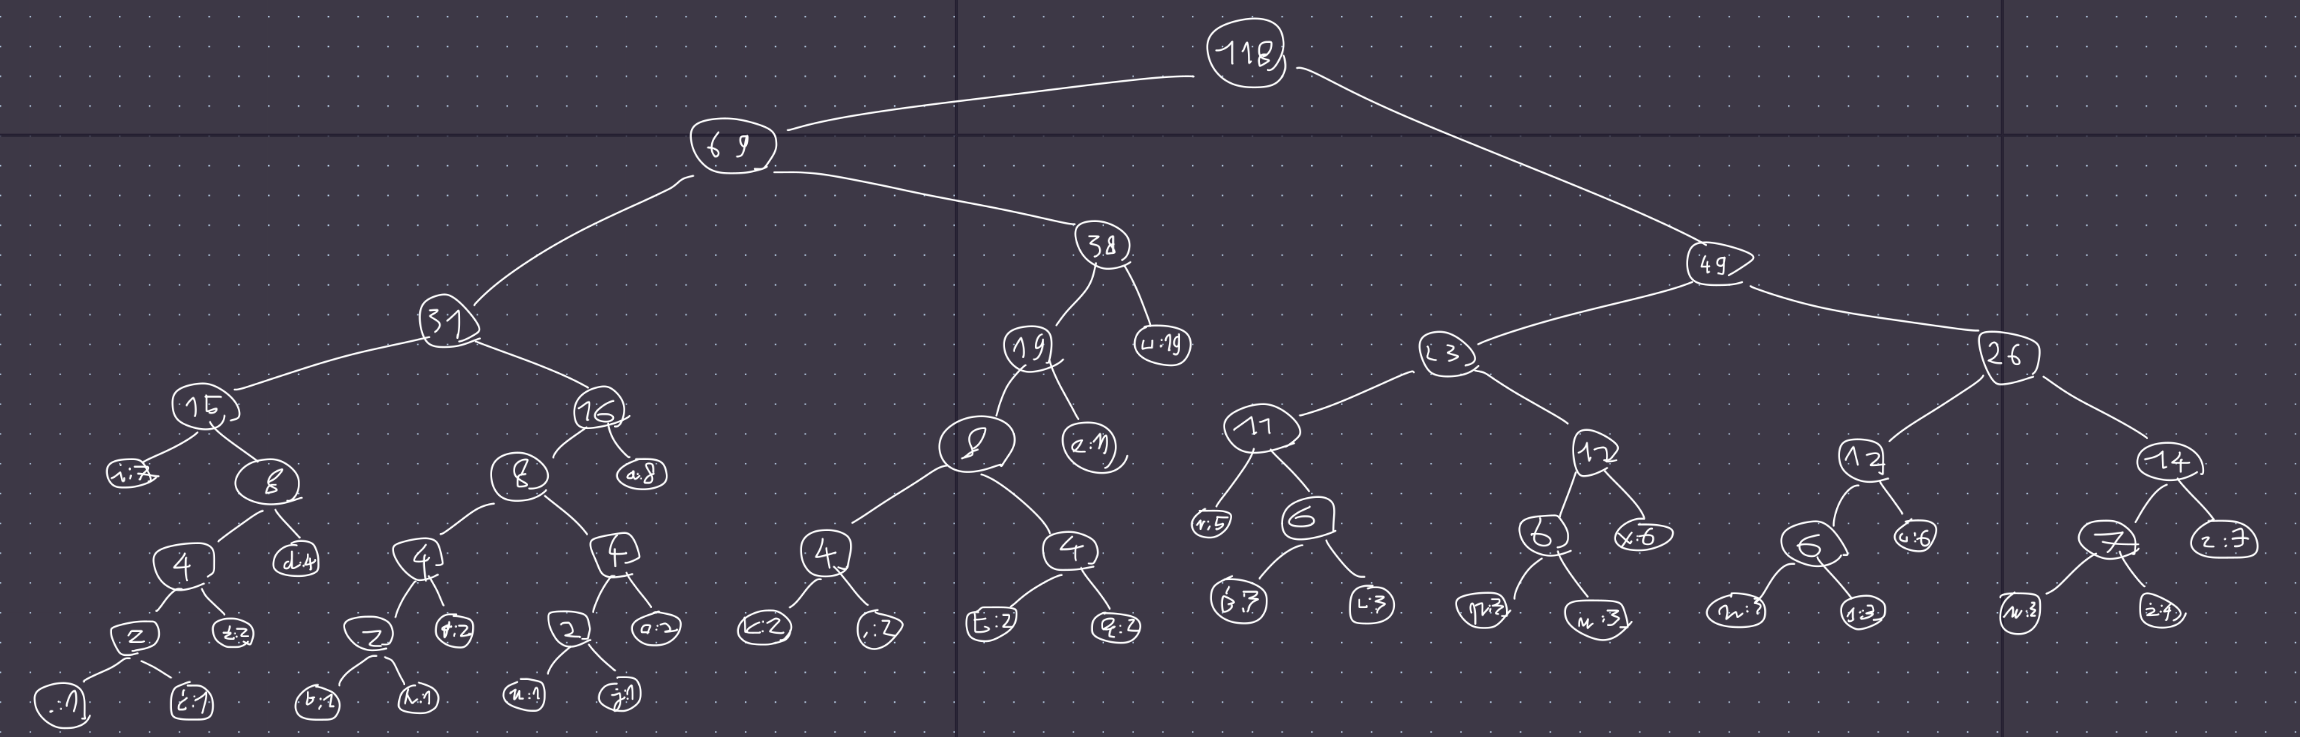
\includegraphics[width=\textwidth]{images/tree.png}
    \caption{Drzewo kodu prefiksowego dla zadania 2.}
    \label{fig:zadanie2-tree}
\end{figure}

K = 3·2 + 5·4 + 3·6 + 7 + 3·8 + 11 + 2·12 + 14 + 15 + 16 + 19 + 23 + 26 + 31 +
38 + 49 + 69 + 118 = 528

\textbf{3.} W pliku poddawanym kompresji występują wszystkie (256) symbole ośmiobitowe z prawie równą
częstotliwością (tzn. symbol występujący najczęściej może wystąpić maksymalnie dwa razy częściej niż 
symbol występujący najrzadziej).
Jaka będzie różnica (zysk w postaci zaoszczędzonych bitów), gdy oryginalny zapis ośmiobitowy zastąpimy 
kodowaniem Huffmana? 
Proszę uzasadnić odpowiedź.

\hl{Miejsce na odpowiedź (wraz z uzasadnieniem):}
Gdy mamy posortowane wartości $p_1 \le p_2 \le \dots \le p_{256}$, to łącząc każdy pośredni
nowy węzeł będzie $p_1+p_2 \ge 2p_1 \ge p_{256}$, czyli trafia na koniec kolejki. To
oznacza, że stworzone zostanie drzewo binarne, które jest pełne i wyważone,
czyli dla 256, będzie miało wysokość 8. Dla pliku o N symbolach koszt, będzie
8*N bitów, czyli tyle samo co w oryginalnym zapisie, czyli zaoszczędzimy 0
bitów.
\newline

\textbf{4.} Czym, w przypadku wyznaczania kodu prefiksowego algorytmem Huffmana, jest własność wyboru zachłannego?

\hl{Miejsce na odpowiedź:}
Własność wyboru tutaj polega na tym, że istnieje optymalny kod prefiksowy, w
którym dwa symbole o najmniejszej częstotliwości są liśćmi tego samego rodzica
i leżą na najniższym poziomie drzewa. Wykonywanie tego kroku nie wyklucza
rozwiązania optymalnego, więc możemy go wykonać w każdym kroku algorytmu.
\newline

\textbf{5.} Dlaczego o algorytmie Huffmana (wyznaczania kodu prefiksowego) 
można powiedzieć, że ma własność optymalnej podstruktury?

\hl{Miejsce na odpowiedź:}
Gdy mamy już połączone dwa symbole o najmniejszej częstotliwości, to możemy od
tego zdobyć optymalne drzewo dla pozostałych symboli zostawiając już to
zbudowane drzewo jako optymalne dla tych dwóch symboli. Czyli jakby budujemy
drzewo wykonując krok po kroku optymalne wybory
\newline

\textbf{6.} W trakcie wykładu, kodując drzewo Huffmana, wykorzystywaliśmy trawersację pre-order.
Czy zamiast tego podejścia można wykorzystać jedną z~dwóch pozostałych metod (in-order, post-order)?
Proszę uzasadnić odpowiedź.

\hl{Miejsce na odpowiedź:}
Post-order może być użyty za pomocą stosu (gdy jest 1 to dodajemy na stos, gdy
jest 0 to łączymy dwa węzły ze stosu pomocniczym i dodajemy na stos). In-order
nie będzie działało, bo nie będzie jednoznacznie odtwarzało drzewa. (gdy mamy
węzły A B C, to kod dla ((A,B), C) jest taki sam jak dla (A, (B, C)),
1[A]01[B]01[C])
\newline

\textbf{7.} Proszę podać przykład tekstu (może być jedno słowo), dla którego algorytm LZW będzie:
(A) lepszy, 
(B) gorszy od kodowania Huffmana.

\hl{Miejsce na odpowiedzi:}
(A)  np. ciąg ABABABABABABABAB... (AB powtórzone n/2 razy n=1e6) Huffman: A=0,
B=1, koszt to 1e6 bitów. LZW: A=0, B=1, AB=2, BA=3, ABA=4 itd. Więc aby pokryć
n znaków potrzeba m w przybliżeniu $\sqrt{2n}$ kodów. Dla n = 1e6, to m = 1414.
Słownik ma wtedy ok 1400 wpisów, więc kod to ok. 11 bitów. Czyli
$\sqrt{2\,000\,000} \approx 1414$ kodów $1414 * 11 = 15554$ bitów, czyli LZW
jest lepszy.

(B) np. ABCDEF Huffman: 6 symboli o wadze 1. czyli koszt to 2*2+4*3=16 bitów.
LZW: 6 kodów pojedynczych po 8 bitów. Czyli 48 bitów, bo nie znajdzie
dopasowania dla żadnego ciągu dłuższego niż 1 symbol.
\newline

\textbf{8.} Załóżmy, że w jakimś tekście \textit{X} symbol \textit{p} występuje znacznie częściej 
niż symbol \textit{k}. 
Słowo kodowe którego z tych symboli będzie krótsze?
Czy zawsze będzie krótsze? Proszę uzasadnić odpowiedź.

\hl{Miejsce na odpowiedź:}
W kodzie Huffmana słowo kodowane symbolu p będzie krótsze lub równe słowu symbolu k. Nie musi być ściśle krótsze. 
Gdyby p miało dłuższy kod od k, to po zamianie ich kodów miejscami średnia długość kodu by się zmniejszyła, więc kod nie byłby optymalny.
\newline

\textbf{9.} Proszę podać złożoność obliczeniową (czasową) operacji dodawania 
elementu do kolejki priorytetowej zaimplementowanej na kopcu. 
Proszę wyjaśnić, z czego wynika podana wartość złożoności obliczeniowej.

\hl{Miejsce na odpowiedź:}
Złożoność to O(logn), bo gdy wstawiamy element do kopca, to dodajemy go na
koniec i potem naprawiamy kopiec w górę, czyli będziemy go przerzucać w górę,
a dlatego, że wysokość kopca to logn, to tyle maksymalnie będzie trwało.
\newline

\textbf{10.} Dla każdego z podanych poniżej słów (w tabeli \ref{table:huffman-tree-cost}.)
proszę zbudować drzewo Huffmana, proszę wyliczyć koszt każdego z tych drzew.
Proszę pokazać odręcznie wykonane wynikowe drzewo (może być w formie wycinka zdjęcia kartki). 
Wyniki proszę umieścić w tabeli \ref{table:huffman-tree-cost}.

\begin{table}[h!]
\begin{tabular}{|c|l|c|c|}
\hline
\multicolumn{1}{|r|}{Lp.} & Słowo    & Graficzna reprezentacja drzewa & Koszt drzewa \\ \hline
1.                        & wandal   & 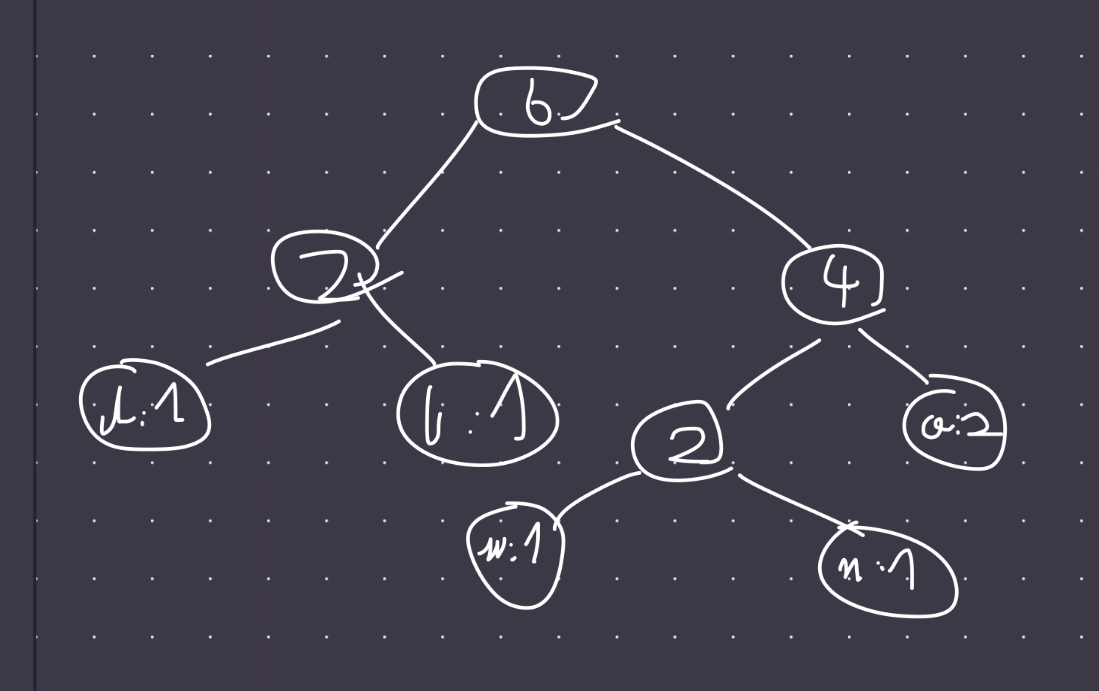
\includegraphics[width=0.28\textwidth,height=0.19\textheight,keepaspectratio]{images/wandal.png}   & 2+2+4+6=14             \\ \hline
2.                        & manna    & 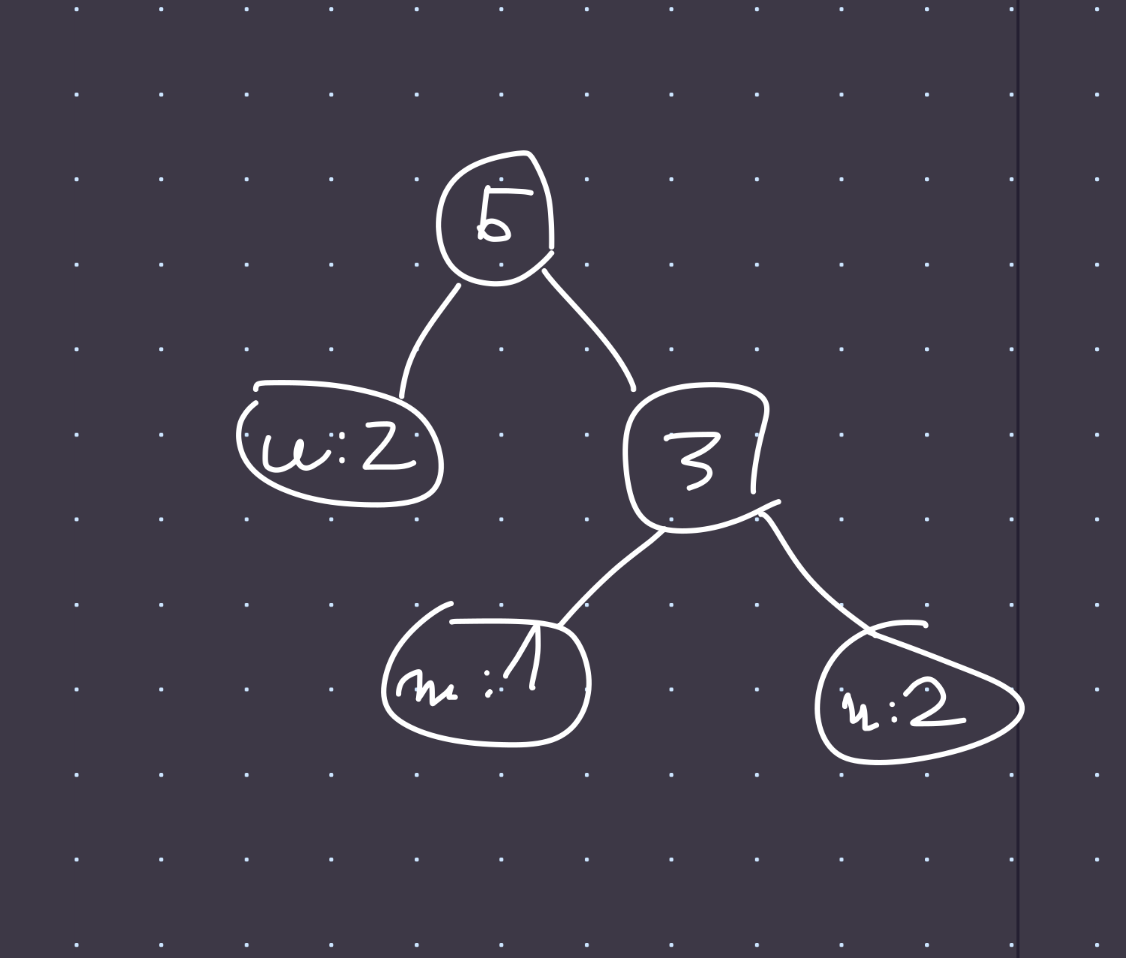
\includegraphics[width=0.28\textwidth,height=0.19\textheight,keepaspectratio]{images/manna.png}    & 3+5=8             \\ \hline
3.                        & wycofana & 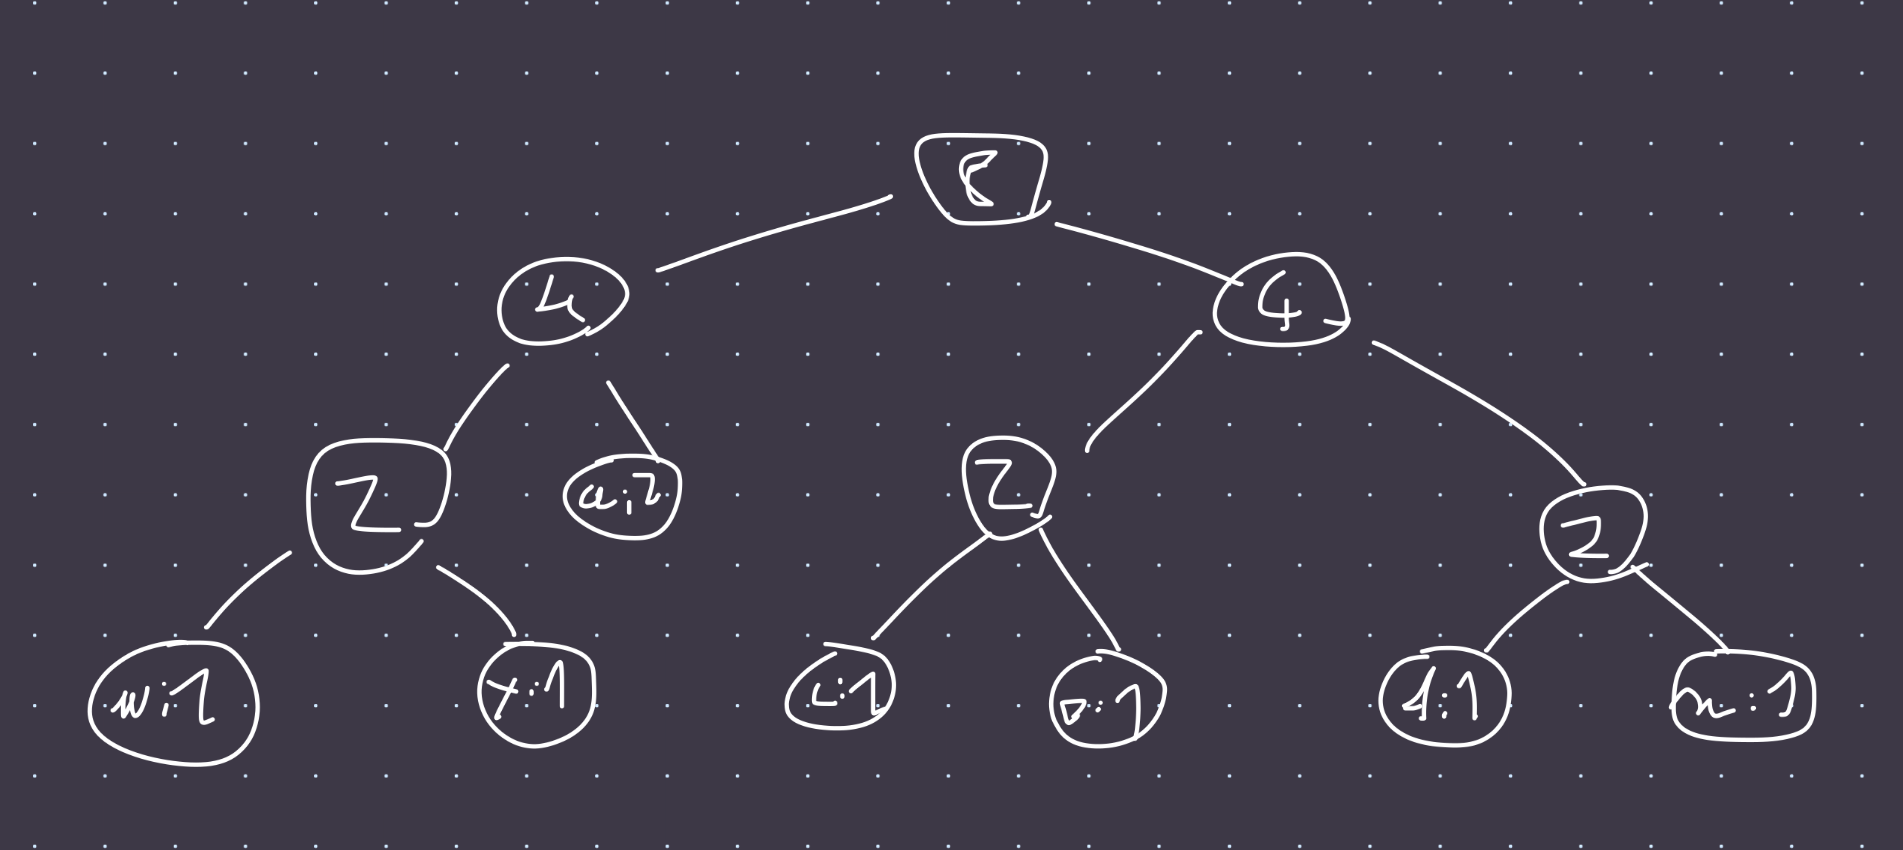
\includegraphics[width=0.28\textwidth,height=0.19\textheight,keepaspectratio]{images/wycofana.png} & 2+2+2+4+4+8=22             \\ \hline
\end{tabular}
\caption{Rozwiązania z wyliczeniem kosztu drzew Huffmana zbudowanych na poszczególnych słowach.}
\label{table:huffman-tree-cost}
\end{table}

\textbf{11.} Czy prawdziwe jest stwierdzenie, że koszt drzewa jest sumą wewnętrznych węzłów drzewa kodowania
(węzłów niebędących liśćmi tego drzewa)? 
Proszę uzasadnić odpowiedź -- najlepiej będzie, jeśli przeprawadzą Państwo dowód dla tej tezy.

\hl{Miejsce na odpowiedź:}
Teza. Koszt drzewa $K(T)=\sum_{c} f(c)\,d(c)$ jest równy sumie wag wszystkich węzłów wewnętrznych drzewa, gdzie waga węzła $w(v)$ to suma częstości liści w poddrzewie o korzeniu $v$.

Dowód. Liść $c$ leżący na głębokości $d(c)$ ma na ścieżce od korzenia dokładnie $d(c)$ przodków i wszystkie są węzłami wewnętrznymi. Zatem liść $c$ należy do poddrzew dokładnie $d(c)$ węzłów wewnętrznych, więc jego częstość $f(c)$ wchodzi do sumy wag węzłów wewnętrznych dokładnie $d(c)$ razy. Stąd
\[
  \sum_{v\ \text{wewn.}} w(v)
  = \sum_{v\ \text{wewn.}} \ \sum_{c \in T_v} f(c)
  = \sum_{c} f(c)\cdot d(c)
  = K(T).
\]

W algorytmie Huffmana każde łączenie tworzy jeden węzeł wewnętrzny o wadze równej sumie łączonych węzłów, więc koszt drzewa jest sumą wszystkich liczb wstawionych do kolejki priorytetowej.
\newline

\textbf{12.} Podczas budowania drzewa kodowania, wykorzystując podejście zachłanne, z kolejki priorytetowej
wybierana jest para dprzykład z wagami 1,rzew, które następnie łączone są w jedno drzewo.
(A) Jeżeli istnieje kilka drzew (więcej niż dwa) o takiej samej wartości w korzeniu, to czym należy się 
kierować podczas wyboru tych drzew?
(B) Czy zmiana kolejności wyboru tych drzew (wyboru dwóch drzew do pary) może wpłynąć na końcową 
strukturę / kształt drzewa?
(C) Czy taka zmiana będzie miała wpływ na końcowy rezultat kompresji (w kontekście kosztu drzewa)?

\hl{Miejsce na odpowiedź:}
(A) Przy remisie wag korzeni wybór jest dowolny: dowolne dwa z drzew o jednakowej, najmniejszej wadze są poprawnym wyborem. Algorytm zachłanny wymaga tylko, by wybrane drzewa miały najmniejsze wagi, a nie wskazuje, które z równych wybrać. (Można przyjąć regułę porządkującą, np. kolejność wstawienia do kolejki, by wynik był deterministyczny.)

(B) Tak, zmiana wyboru może zmienić kształt drzewa, a więc długości słów kodowych i ich przypisanie symbolom. Przykład: wagi $1,1,2,2$. Po połączeniu $1+1=2$ w kolejce są trzy dwójki i można:
\begin{itemize}
  \item połączyć dwa liście o wadze $2$: powstaje $4$, potem $2+4=6$. Wszystkie kody mają długość $2$ (długości $2,2,2,2$);
  \item połączyć węzeł $(1,1)$ z liściem o wadze $2$: powstaje $4$, potem $2+4=6$. Długości kodów to $1,2,3,3$.
\end{itemize}

(C) Nie, koszt drzewa pozostaje taki sam. Każdy taki wybór jest zgodny z własnością wyboru zachłannego, więc prowadzi do drzewa optymalnego, a wszystkie drzewa optymalne mają tę samą, minimalną wartość
\[
  K(T)=\sum_{c} f(c)\,d(c).
\]
W przykładzie z (B) w obu przypadkach $K = 2+4+6 = 12$ (sprawdzenie: $1\cdot2+1\cdot2+2\cdot2+2\cdot2=12$ oraz $2\cdot1+2\cdot2+1\cdot3+1\cdot3=12$). Zatem różne drzewa Huffmana dla tych samych częstości mogą różnić się kształtem, ale mają identyczny koszt, czyli identyczną długość skompresowanego tekstu. tekstu.
\newline

\textbf{13.} Ciągi składające się z symboli \verb|0| i \verb|1| można tworzyć wykorzystując 
m.in. słowa: Thuego-Morse'a, Cantora, Fibonacciego, \href{https://googlethatforyou.com?q=Regular%20paperfolding%20sequence}{Paper-folding} (składania kartki papieru).

\begin{table}[h!]
\begin{adjustwidth}{-1in}{} 
\begin{tabular}{|l|l|p{1.5cm}|p{1.5cm}|l|p{5cm}|}
\hline
Lp. & Nazwa & Pierwsze (zerowe) słowo & Drugie słowo & Trzecie słowo & Opis wyliczania i-tego słowa \\ \hline
1. & Thuego-Morse'a & 0 & 01 & 0110 & Każde kolejne słowo zastępuje znaki w poprzednim słowie. 0 -\textgreater 01; 1 -\textgreater{}10. \\ \hline
2. & Cantora & 1 & 101 & 101000101 & Pierwszym słowem jest 1. Każde kolejne słowo powstaje przez zastąpienie symboli poprzedniego słowa: 0-\textgreater{}000, 1-\textgreater{}101. \\ \hline
3. & Paper-folding & 1 & 110 & 1101100 & W każdym kroku zginamy kartkę papieru w prawo. Po wykonaniu n zgięć zapisujemy powstałe zgięcia. Jeśli jest zgięcie w prawo, to zapisujemy 1, a jeśli w lewo -- 0. \\ \hline
4, & Fibonacciego & 1 & 0 & 01 & Początkowym słowem jest 1. Kolejne słowa powstają przez zastąpienie symboli poprzedniego słowa: 0-\textgreater{}01, 1-\textgreater{}0. \\ \hline
\end{tabular}
\end{adjustwidth}
\caption{Skrócony opis wybranych słów nad alfabetem syboli binarnych.}
\label{table:words-transform-description}
\end{table}

Dla podanych definicji tworzenia słów \ref{table:words-transform-description}, proszę uzupełnić tabelę \ref{table:words-transform-results}.
\newline

\begin{table}[ht!]
\begin{tabular}{|l|l|l|}
\hline
\multicolumn{1}{|r|}{Lp.} & Opis                                                        & Wynik \\ \hline
1.                        & Piąte słowo Cantora kompresowane przez algorytm RLE         &       \\ \hline
2.                        & Wynik TBW przeprowadzonej na piątym słowie Thuego-Morse'a   &       \\ \hline
3.                        & Wynik algorytmu MTF na szóstym słowie Fibonacciego          &       \\ \hline
4.                        & Wynik TBW przeprowadzonej na piątym słowie Paper-folding    &       \\ \hline
5.                        & Wynik algorytmu MTF przeprowadzonego na wyniku z wiersza 4. &       \\ \hline
6.                        & Wynik algorytmu RLE przeprowadzonego na wyniku z wiersza 5. &       \\ \hline
\end{tabular}
\caption{Rozwiązania przekształceń wykonanych na słowach symboli binarnych.}
\label{table:words-transform-results}
\end{table}

\textbf{14.}
Proszę pokazać wyniki działania transformaty Burrowsa-Wheelera na napisie powstałym z połączenia własnego 
imienia i nazwiska. 
Proszę pokazać dwa warianty rozwiązania.
\newline

\hl{Miejsce na odpowiedź: .....TODO}

\end{document}
